

\section{A new Emulation Technique for Sensitivity Analysis
for SRAM FPGAs}
\label{intro}
% no \IEEEPARstart


This work addresses to make the FPGA based emulation platform that imitates the radiation based experiment. In this work, the signature is calculated that presents the faulty behavior of the computation. The new fault emulation technique is used, this method is based on the bits relative sensitivity, and it's feature. The purpose to use the sensitivity specific bits to produce the highly accurate fault behavior as expected in the real-time testing environment.  We observed that the signature computed by our sensitivity-based method are $98.47$\% closer for adder circuit and $99.49$ \% closer for the multiplier circuit to the radiation based signature.

Space is not the only environment where radiation is found. Indeed, it has already been proved that the integrated circuits can also be affected by the radiations at the commercial flight altitudes~\cite{normand1996single}. At ground level, the effect of the radiations can be felt, although this effect is much less than the effect in space\cite{normand2004single}. As a result, the field of aeronautics has been concerned for the consequences of cosmic radiation. Studies to investigate the sensitivity of avionics-based electronic devices to induced particle bombardment are increasing~\cite{bagshaw2008cosmic}.
The potential analysis of a malfunction due to radiation encourages manufacturers to invest more and more in the development of the design tools that allows the choice of the mitigation strategies. On the other hand, verify the estimation of the resulting reliability. In the 1980s,
components have begun to be developed for space applications and Aviation
In the 1990s, the explosion of the development of consumer electronics multiplied
Commercial Off-The-Shelf (COTS) components, which are increasingly
economic and available in large quantity. Further,  the reduction
of the transistor sizes, the intrinsically small transistor is less sensitive to
radiation. But because of its smaller sensitive surface, the opposite effect is observed at the level of an integrated circuit. Indeed, the sensitivity of the components increases while the ability of
engraving decreases despite the gain brought by the miniaturization. The two main factors
of this conjecture are the increase in the density of integration and the
threshold voltages of the transistors. For the last ten years or so, studies have been able to provide the evidence of the potential sensitivity of integrated circuits at high altitude commercial flights \cite{normand1998extensions}. This is particularly the case for complex components with high integration such as
those based on Static Random Access Memory (SRAM) \cite{baumann2005radiation}, which is the target technology for this project. The aerospace industry is looking for the solutions that offer an acceptable compromise between radiation reliability and the system cost, including those based on user-programmable integrated circuits based on static memory. The search for such solutions has implications for the complete flow of design and development of embedded systems. Indeed, this requires the designers to check design robustness to the radiations design. For this purpose, simulation tools that allow the injection of faults in the design is being used. But simulation-based verification has its limits, long testing time is added to the conventional verification, which is already considered to the bottleneck of the design process. The system, once implemented, should also be subject to costly laboratory testing using particle accelerators. To provide a cost-effective pre-certification process, the fault emulation techniques were developed by our research group ~\cite{hobeika2014multi,  bocquillon2009evaluation,souari2015optimization}. The purpose of these techniques is to reproduce as close as possible radiation based test results. In this work, we extend the previous work and make the following contributions. \\



%Considering the costs of this certification and the limitations of fault simulation, it becomes imperative to maximize the chances of success of so-called pre-certification tests. In the process of developing a system to be certified, these tests are performed once the system is implemented but before it is sent for certification. The implementation of such tests, which must be representative of those carried out during the certification, will have an impact on the design and development flow. In the 1980s, for example,
%components have begun to be developed for space applications and Aviation.
%In the 1990s, the explosion of the development of consumer electronics multiplied
%commercial Off-The-Shelf (COTS) components, which are increasingly
%economic and available in quantity. This race is made possible by the reduction
%of the transistor sizes. If intrinsically a small transistor is less sensitive
%radiation, because of its smaller sensitive surface, the opposite effect is observed at
%level of an integrated circuit. Indeed, the sensitivity of the components increases while the ability of
%engraving decreases despite the gain brought by the miniaturization. The two main factors
%of this conjecture are the increase in the density of integration and the
%threshold voltages of the transistors. For the last ten years or so, studies have been able to
%evidence of the potential sensitivity of integrated circuits at high altitude avionics \cite{normand1998extensions}
%and even at the ground level where the neutron flux is 300 times lower than that encountered by the flights
%commercial. This is particularly the case for complex components with high integration such as
%those based on Static Random Access Memory (SRAM) \cite{baumann2005radiation}, in which
%appear new effects like the MBUs (Multiple Bit Upsets) and MCUs (Multiple Cells
%Upsets), until recently little or not met. On the other hand, hardened components, which did not benefit from the same demand, developed more slowly. This added to the
%reduction in the budgets of space projects, the trend since the
%the use of COTS components in space and aeronautical applications \cite{diubaldo2000nasa}.
%%The market for complex COTS circuits is divided into two main categories: components
%ASICs (Application-Specific Integrated Circuit) that are dedicated circuits and components
%reprogrammable FPGA (Field-Programmable Gate Array). ASICs generally offer
%better performance and less energy consumption than FPGAs. For their part, the
%FPGAs are valued for their low cost, good performance, short
%market and their great flexibility during development. In addition, FPGA models based on
%SRAM type configuration memory are particularly suitable for space applications and
%aeronautics thanks to their ability to reconfigure themselves on site. Despite these characteristics,
%the designers of embedded systems are often reluctant to use this type of
%component for critical applications because the profiles of the missions in which they
%often include a severe radiative environment. Radiation-related phenomena
%the most commonly encountered on SRAM-based FPGAs are SEUs and MBUs
%which can affect the memory used by the application (for example a flip-flop, a
%state machine, storage memory, etc.) or the configuration memory. In the first
%case a simple reset of the application makes it possible to return to normal operation. By
%a fault in the configuration memory is retentive, that is, it is
%permanent until the FPGA is reconfigured. In addition, this bit inversion can result in
%a mutation of the logic functions implanted in the component leading to
%unpredictable and potentially critical.
%Due to their possible dangerousness, the upsets in the configuration memory of the FPGA
%must be taken into account by designers of critical applications that require a high
%level of reliability in the radiative medium.  Before sending the device in the radiation concerns environment fault emulation techniques are extensively reported in the literature~\cite{alderighi2003fault},~\cite{manuzzato2010single}. 


%A technique to mitigate errors due to radiation
%is known as TMR (Triple Modular Redundancy) \cite{kastensmidt2005optimal}, is often adopted
%making applications more robust. This methodology consists in performing in parallel three times
%the same operation thanks to three identical and independent operators, a majority voting
%then determines the correct result. In theory, the weak point of TMR is its comparator
%since triplication can not protect it. Moreover, the persistence of faults in the
%configuration memory causes an upset build-up phenomenon that can corrupt
%the functionality of several calculation operators and thus to check the TMR.
%

\textbf{Contributions:} \\

\begin{itemize}


%\item{This work presented a methodology for modeling the faulty behavior of digital circuits. In this work, the abstract high-level model/mathematical representation of the signature is presented. This signature model is constructed for the FPGA-based circuits and can be described at a high-level of abstraction.}  

\item{Developed a realistic fault emulation technique in the configuration memory
of FPGAs based system. The purpose of realistic emulation system is to produce
the emulation results close to those obtained by certification tests under
radiation}.

\item{In this work, we propose a fault injection method by using relative sensitivity values between the bits features: e.g., bits belong to LUT at "0", bits belong to LUT at "1", bits belong to Non-LUT at "0", bits belong to Non-LUT at "1"}.

\item{Zero-siganture has been derived by flipping the bits-at-1, bits-at-0, random, relative sensitivity between bit-at-1, bits-at-0, and relative sensitivity between bits-status and their features}.
\end{itemize}

%In this work, we developed a high-level mathematical models that represent the faulty behavior of digital circuits. The modeling of the faulty behavior of the circuit could be beneficial for the designers to take the necessary mitigation measures for the design in the appropriate abstract level before sending the design in an environment that is harsh for the electronic components, e.g., aircraft flying at the altitude of 50,000 ft.

In order, to find the faulty behavior of the circuits for their early validation, we extracted the information from the arithmetic signatures in terms of zero-signatures. To emulate faults in the FPGA based design, we  developed a suitable fault injection method. The fault injection method is based on the relative sensitivity of the bits and bits features as well, i.e., the bits belong to look-up-table or non look-up-table bits. We observed that by considering the bits feature; we produced more realistic results closer to the real-time experiments. In this paper, we also provide the results if the sensitivity of the bits is not taking into consideration lead towards the deviated results for the real-time radiation experiment.


\section{Related Work}




%This section discusses the fundamental concepts and current research in different areas related to this work: radiation enviornemnt, radiation effects on SRAM-FPGAs, soft-error, hard-error, Fault-injection, Signatures,  and radIation testing. In this section, we also describe the radiation present in both space and in the Earth's atmosphere and their interaction with integrated circuits mainly neutrons interactions with the semiconductor.
%\subsection{Environment and radiation sources}
%The spatial radiative environment comes from different sources such as
%Van Allen radiation, solar activity, and cosmic radiation. Each offers a variety of particles, and each type of particle cause different types of  effects on
%electronic components, e.g., 
%the electrons and protons of the radiation belts, as well as the protons
%ejections of the coronal mass of the sun, resulting in a total dose effect on the integrated circuits~\cite{Boudenot2007}. The
%cosmic radiation and charged particles ejected by solar flares are responsible
%singular events~\cite{Boudenot2007}.


%\subsection{Ejections of Matter by the Sun}
%Here we distinguish two types of phenomena concerning the radiative environment:
%\begin{itemize}
%
%
%\item{Coronal Mass Ejection (CME - Coronal Mass Ejection) is a plasma bubble that
%to reach several tens of solar rays. These phenomena mainly emit high-energy protons.}
%\item{The solar flare is a jet of ionized matter amounting to hundreds of thousands of
%kilometers of altitude. These are heavy, high-energy ions.}
%
%\end{itemize}



%\subsection{The Solar Wind}
%The solar wind begins in the solar corona, where temperatures are in million degrees. This gives the electrons enough energy to allow them to
%escape from the gravitational field of the Sun. In reaction, protons and heavy ions are also ejected so that the sun retains a zero electric charge. The Sun evacuates about $10^{14}$ kilograms of material each day. This flow of plasma projected in all directions
%hit the Earth at speed between $300$ and $1000$ $km / h$.
%
%

%Cosmic radiation refers to the flow of high-energy particles
%from the universe. It is composed of 87\% protons, 12\% helium nuclei, the remainder being mainly
%heavy ions. The low-energy particles originate from the Sun, those of medium-energy supernovas (these are galactic phenomena) and neutron stars. The particles of
%very high energies correspond to gamma-ray bursts and galaxy collisions; they are
%extra-galactic phenomena (the highest detected energy is $10^{20} eV$). There are
%particles of the solar system, and even the earth's magnetic field is
%often insufficient to divert them.
%
%\subsection{Van Allen Radiation Belts}
%The Van Allen radiation belts are two toroidal zones of the magnetosphere
%magnetic field surrounding the magnetic equator and containing a high particle density
%Energy. The magnetosphere is the region surrounding a celestial object in which the
%physical phenomena are dominated or organized by its magnetic field. It is located above
%beyond the ionosphere, that is to say above $800$ to $1,000$ $km$ of altitude. This area of ​​space
%acts as a real protective shield against radiation. Indeed the solar winds
%strike the magnetosphere to form a drop of water; a small
%part of the particles is trapped by it while the greater quantity is rejected on the
%sides. The periods of intense solar activity give rise to magnetic storms and
%polar aurora (boreal or southern) by particles that penetrate the atmosphere by
%the poles. The distribution and type of particles vary according to geographical position and altitude. The
%the most important disturbance in their arrangements is the South Atlantic Anomaly (SAA -
%South Atlantic Anomaly) where these belts come within $500$ $kms$ of the Earth. Both
%Van Allen's radiation belts are composed of "inner belt" and "outer belt."
%

%These previously mentioned sources of particulate matter affect only persons and equipment
%outside the Earth's atmosphere. However, since 1992, the year of observation of the first
%bit-flipped in an atmospheric flight memory, hundreds of similar effects could be recorded
%over several hundred flights (civil and military) corresponding to several
%thousands of flight hours. It has been demonstrated that the particles responsible for these
%phenomena are atmospheric neutrons ~\cite{leray2004atmospheric}.
%Atmospheric neutrons are the result of the collision of cosmic radiation,
%mainly protons, with the atoms present in the upper atmosphere of the Earth~\cite{guenzer1979single}. The result of these collisions is either the formation of ionized particles or a nuclear reaction which
%produced mainly neutrons, protons, electrons, etc. These phenomena are called
%"Atmospheric shower" \cite{ziegler1996ibm} shown in Figure~\ref{shower}. The product resulting from these collisions is the generation of
%protons, neutrons, muons, etc. Since neutrons are uncharged particles, they do not
%cause  - directly operational failure of electronic devices. On the other hand, they can generate kernels of recoil in
%the material they cross. When these ions originate in the active zones of the integrated circuit, they are able to modify the normal behavior of the components~\cite{normand1998extensions}.
%%
%
%
%\begin{figure}[h]
% \centering
%  \captionsetup{justification=centering}    
%   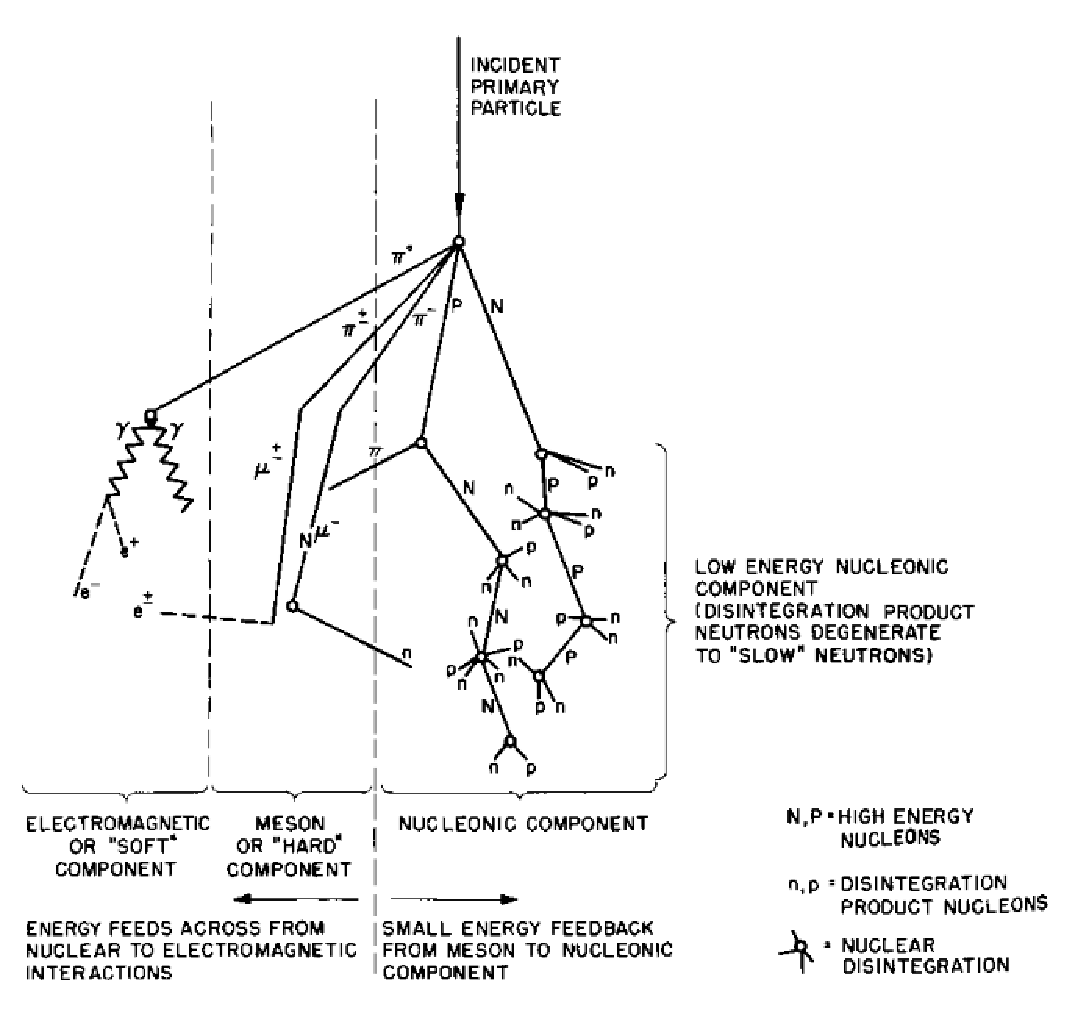
\includegraphics[scale=0.5]{figures/neutron.pdf}
%  \caption{Cosmic rays shower~\cite{ziegler1996ibm}.}
%\label{shower}
%\end{figure}
%
%
%\subsection{Neutron interactions}
%The neutron is a particle without electric charge but with mass. By penetrating into
%the material a particle encounters a lot of vacuum, and in case of impact, it mostly strikes electrons\cite{normand1998extensions}. Therefore, the probability that a neutron interacts is varied. However, indirect effects are significant. Indeed, it can only be stopped by a
%collision with a nucleus during a spallation reaction, which releases very light particles
%ionizing. During the collision various phenomena can occur, the three most important ones are the following:
%\begin{itemize}
%
%\item{Elastic scattering: the incident neutron imparts a part of its energy to the atom
%which can leave its crystalline mesh if the energy it receives is sufficient.}
%\item{Inelastic scattering: the atom captures the incident neutron, recovers part of its
%then release it. The excited atom can then return to its original state by
%the emission of a ray $\gamma$, but in general, it leaves its crystalline mesh and interacts.}
%\item{Transmutation: The incident neutron is absorbed by the nucleus of the atom struck. The particle moves into another atomic element. This effect is not significant except in the
%particular where the neutron comes into contact with a boron atom (used for doping
%of substrates in CMOS technology). The latter disintegrates by emitting an $\alpha$ particle and
%a lithium $7$ atom, which may interact in turn.}
%Neutrons are classified into three categories according to their energy: slow neutrons
%$(<1$ $ $ $eV$$)$ including thermal neutrons $(26$ $ $$meV$$)$, intermediate neutrons (between $(1$ $  $$meV$$)$ and
% $(100$ $ $$keV$$)$ and fast neutrons $(>$$100$ $ $$keV$$)$.
%
%
%\end{itemize}
%
%
%%\section{Related Work}
%
%
%%This section discusses to the fundamental concepts and current research in different areas related to this work: radiation effects on SRAM-FPGAs, soft-error, hard-error. Fault-injection, Signatures,  and radation testing.
%
%\subsection{Single Event Effects Mechanism}
%
%A Single Event Effect (SEE) results from a single energetic particle. When the particle strikes a sensitive node in a semi-conductor device, the ionization by the particle might produce a current pulse inside the device, which might cause soft or hard errors in the configurtaion memory of the device. Results in data corruption, transient disturbance, high current conditions (non-destructive and destructive
%effects). SEE can if not handled well cause unwanted functional interrupts or in worst case catastrophic failures. Commonly, SEEs include single event upset (SEU), single event latch-up (SEL), single event burn-out (SEB), and single event transient (SET) etc. a
%
%
%%
%%\begin{table}
%%\caption{Single Event Effects Summary}
%%\centering
%%\label{SEE-Summary}
%%\scalebox{0.4}{
%%
%%   \begin{tabular}{c|c|c}
%%         \toprule
%%    \hline
%%     
%%     Single Event Upset (SEU)                  & corruption of the information \\ & stored in a memory element            & Memories, latches in logic devices                                  \\ \hline
%%    
%%    Multiple Bit Upset (MBU)                  & several memory elements \\ & corrupted by a single strike                & Memories, latches in logic devices                                  \\ \hline
%%    Single Event Functional Interrupt (SEFI) & corruption of a data path      & Complex devices with built-in state       \\ \hline
%%    Single Hard Error (SHE)                   & unalterable change of state in\\ & a memory element                     & Memories, latches in logic devices                                 \\ \hline
%%    Single Event Transient (SET)              & Impulse response of certain\\ & amplitude and duration                  & Analog and Mixed Signal circuits                      \\ \hline
%%    Single Event Disturb (SED)                & Momentary corruption of the\\&information stored in a bit             & combinational logic, latches in logic devices                       \\ \hline
%%    Single Event Latchup (SEL)                & high-current conditions                                              & CMOS, BiCMOS devices                                                \\ \hline
%%    Single Event Snapback (SESB)              & high-current conditions                                              & N-channel MOSFET, SOI devices                                       \\ \hline
%%    Single Event Burnout (SEB)                & Destructive burnout due to\\ & high-current conditions                  & BJT Power MOSFET    \\ \hline
%%    Single Event Gate Rupture (SEGR)         & Rupture of gate dielectric due\\&to high electrical field\\ & conditions & Power MOSFETs \\ \hline
%%    
%%    \bottomrule
%%    
%%    \end{tabular}
%%    }
%%\end{table}
%%
%%
%%
%
%
%
%


FPGAs are complex reconfigurable devices that comprise a wide family of different resources. The basic structure of modern FPGAs includes interconnect resources, clock-management resources, configurable logic blocks (CLBs), input/output
blocks (IOBs), and embedded blocks such as digital signal processors (DSPs), general-purpose processors, high-speed IOBs, and memories. CLBs are used to perform simple
combinational and sequential logic. These blocks are typically formed of look-up tables
(LUTs), multiplexers, flip-flops, and carry logic. Programmable interconnect resources, such
as routing switches, allow interconnecting CLBs, IOBs and embedded blocks to implement multiple systems.
The logic and routing resources in an FPGA are controlled by the bits of a configuration memory, which may be based on either antifuse, flash, or SRAM technology. 

%The
%design flow of FPGA-based systems as shown in Figure~\ref{fig:fpga-struct} adapted from ~\cite{hauck2010reconfigurable} involves the creation of a bitstream to load into the
%device.
%
%
%
%\begin{figure}[tb!]
% \centering
%  \captionsetup{justification=centering}    
%   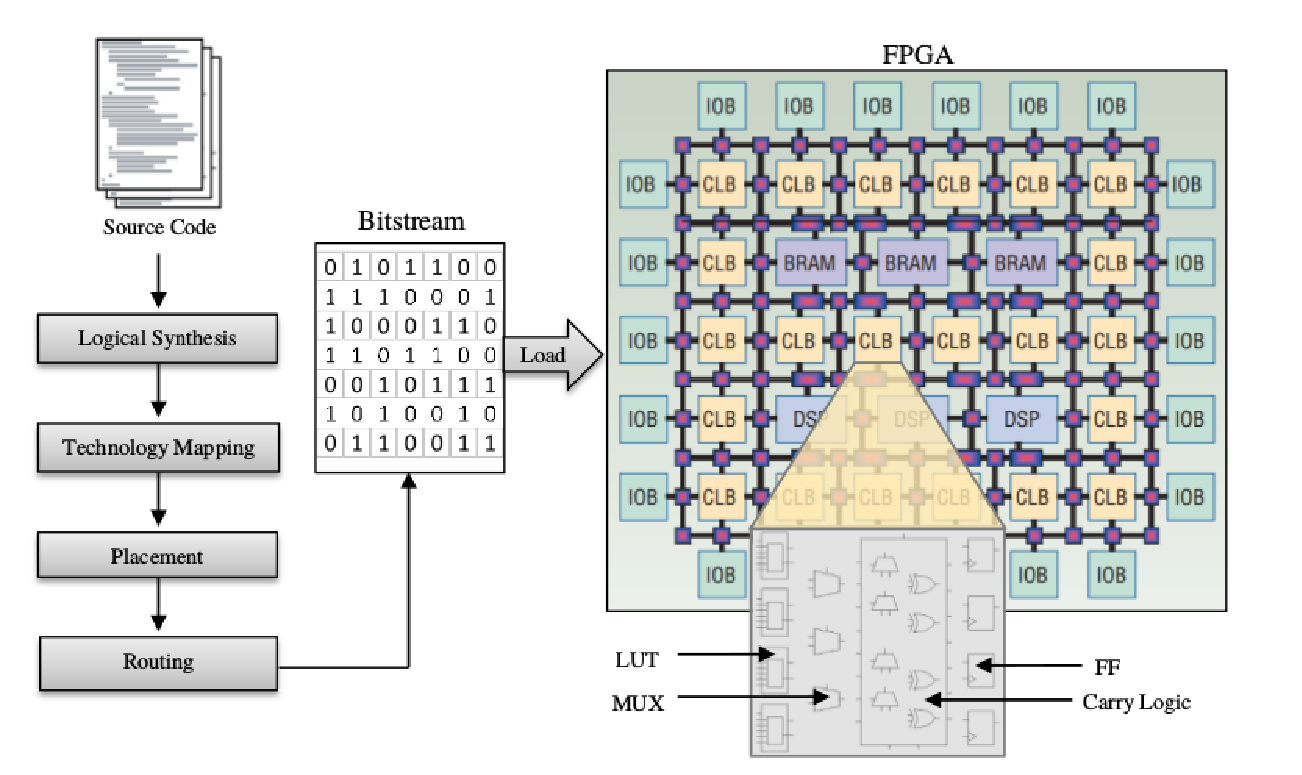
\includegraphics[width=6cm, height=4cm]{figures/FPGA-structure.pdf}
%   \caption{FPGA Structure and Design Flow~\cite{manuzzato2010single}.}
%\label{fig:fpga-struct}
%\end{figure}


In such devices, this memory may represent more
than 80 percent of the total memory bits, increasing the probability of configuration faults.
Upset configuration bits may change the logic and routing of the implemented system, as
shown in Figure~\ref{fig:seu}, leading to functional failures in an unpredictable way. In contradiction, the primary concern for anti-fuse and flash-based FPGAs is SETs and SEUs within user flip-flops
and block memories. However, the configuration memory blocks of anti-fuse and flash-based
FPGAs offer a relative immunity to SEEs, but these devices have lower logic capacity and
cannot be reprogrammed an unlimited number of times, making SRAM-based FPGAs more
suitable for complex systems requiring frequent reconfiguration and adaptation~\cite{quinn2015validation, violante2004simulation}.

\begin{figure}
 \centering
  \captionsetup{justification=centering}    
   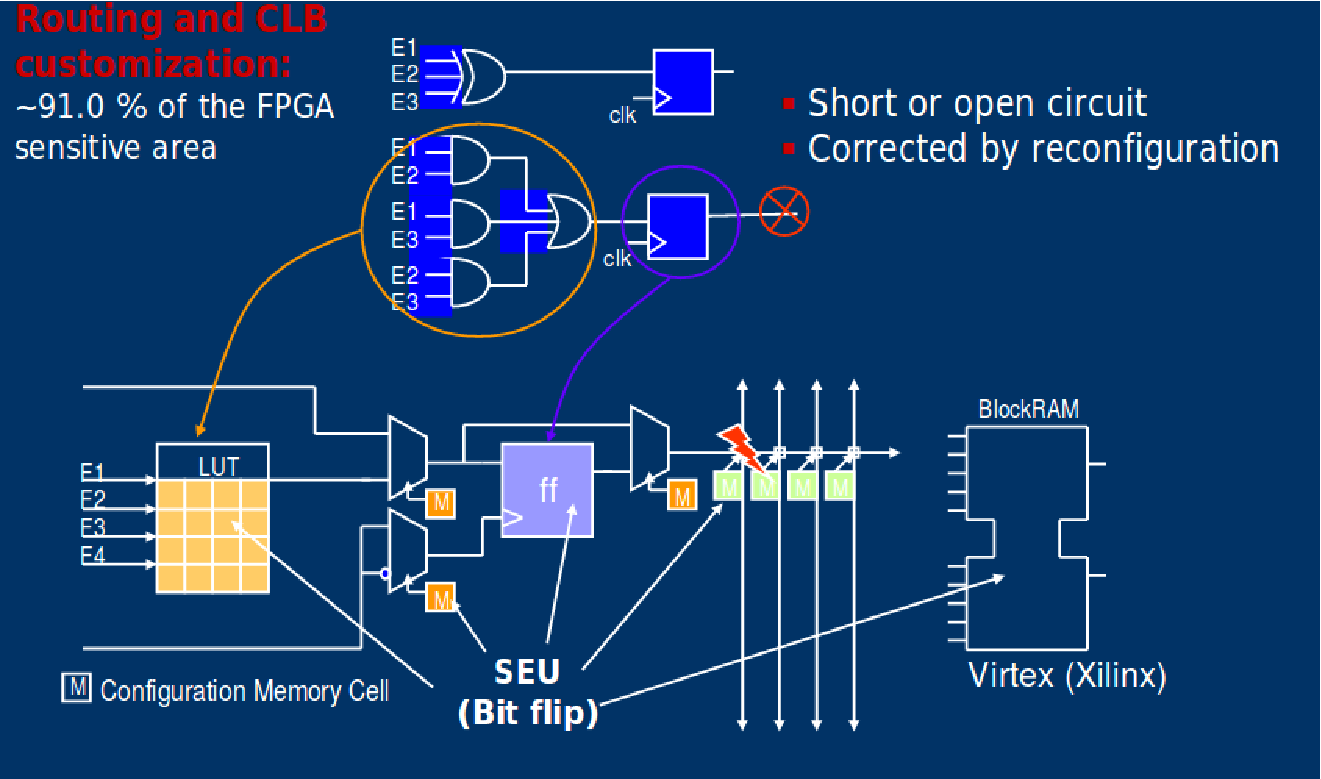
\includegraphics[width=8cm, height=4cm]{Figures/seu.pdf}
   \caption{Upset FPGA configuration bits may change the logic and routing~\cite{manuzzato2010single}.}
\label{fig:seu}
\end{figure}





The SRAM-based FPGAs are particularly sensitive to single event upsets (SEUs). The configuration memory is the most sensitive part, by changing the configuration memory, may affect the overall functionality of the system. The work have done so far deal the SEU effects on FPGAs, combines the simulation, radiation, and emulation testing~\cite{quinn2015validation, violante2004simulation, hobeika2014multi, robache2013methodology, quinn2015using, souari2015optimization}. These papers described how they make the faulty behavior of the system to build an accurate representation of the system. The work presented in~\cite{quinn2015using} described the benchmark that can be used for the reliability and radiation effects study on FPGAs and microprocessors. FPGAs offer high densities and run-time programmability facility make inconvenient to use in the aerospace domain. But, FPGAs are sensitive to high-energy ions.  We need to study the sensitivity of SRAM-based FPGAs to heavy ions that show the suitability and analysis of effects of radiation on FPGAs when employed in space, e.g., usage of FPGAs in aircraft. The work presented in~\cite{hobeika2014multi} investigate the sensitivity of SRAM-based FPGAs devices not only for the simulation-based approach but also used emulation and radiation testing for evaluating the effects of SEUs. The work presented in~\cite{souari2015optimization} described the fault injection emulation in Xilinx FPGA based on the identification of critical configuration bits. Based on SRAM-based FPGAs, two aspects can be considered:

%\subsection{Emulation}
%The emulation of SEUs in an FPGA is done by flipping the bit in the configuration memory. The emulation can be done by using the IP provided by the Xilinx named - SEM core. The work adopted the emulation work also proposed in the~\cite{hobeika2013flight}.  The work described a completed automated methodology to emulate SEUs on an FPGA efficiently. The work presented in~\cite{hobeika2014multi} used the Artix-7 board for the emulation puposes. 
%
%
%
%
%The hardware setup consists of two Artix-7 board. Board A used as a reference and board- B is subjected to radiations. The board-A is not bombarded, and it hosted the counters, reference design error detection and signature computation, memories to store signatures and communication controller. 

%A total 20 runs performed on the adder and 14 on the multipliers. Arithmetic errors for both approached DSP and LUT are observed (151 vs. 291 for DSP). This is due to DSP strategy; SEUs can add registers in the data path, leading to the sequential type of errors. The authors in this work compare the results from the fault simulation, fault emulation, and radiation testing. The purpose is to express as signatures, intended to reproduce the faulty behavior. They showed that simulation and emulation based signatures could contain the same error values as obtained with radiation but their probability of occurrence could significantly different. The arithmetic signature for TRIUMF to emulation is 85.3 % for 

\section{Methodology}
\label{Methodology}



The emulation of SEUs in an FPGA is done by flipping the bit in the configuration memory. The emulation can be done by using the IP provided by the Xilinx named - SEM core~\cite{xilinx}. The Xilinx SEM core is used to get the bit flip in the configuration memory of the FPGA. The emulation platform used in this work was designed for the radiation experiment as discussed in section~\ref{intro}. In this work, this platform is employed for the fault emulation. The platform comprises of two Artix-7 FPGAs. The "Referenc-Board" comprises of the original design, e.g., 16-bit adder and 8-bit multiplier. The design under "Test -Board" is subjected to fault emulation.  

%The work adopted the emulation work also proposed in the~\cite{hobeika2013flight}.  The work described a completed automated methodology to emulate SEUs on an FPGA efficiently. The work presented in~\cite{hobeika2014multi} used the Artix-7 board for the emulation puposes. 



This research work comprises of four-step:
\begin{itemize}
\item{Fault emulation platform: configuration and validation}
\item{Fault emulation: flip-at-1, flip-at-0, random fault injection, sensitivity aware, and sensitivity aware based on the bits feature}.
 %\item {High-level fault modelling}
\item{Result analysis and bit flip validation}.
\end{itemize}


The bit flip causes the malfunctioning of the design, and generate the erroneous output behavior of the circuit. To catch the erroneous output behavior of the circuit and corresponding bit that cause that error, two outputs were generated a) Original output (without fault) b) Faulty output (under bitflip). Then the formula as expressed in equation~\ref{eq:1} is used that computes the difference between two boards results if the calculated output is zero revealed no error generated, and the corresponding bit is not critical, if the difference between them is either greater than or less than numeric zero, signature is recorded in the BRAM. The signature is computed based on the difference between the two ouptputs.

\begin{equation} \label{eq:1}
\textit{Arithmetic Signature = Faulty \textsubscript{output} - Original \textsubscript{output}} 
\end{equation}

\subsection{Identification of the Sensitivity bits}
\label{SE-bits}

The most important part of this work is the identification of the bits (the bit address and the bit location). During the experiment, we observed the difference between the \textit{.ebc} file or the \textit{.rbd} file. These files are not equivalent as not the case with Virtex-V. The work presented in the~\cite{souari2015optimization} based on the Viretx-V where authors fault emulation experiment and all the bits information were based on the \textit{.ebc} file of the design marking the bottleneck of the work. Whereas, for Artix-7, we observed a distinction between these two files. This is also another technical contribution of this work as Xilinx changed their technology, need to develop new tools for newer FPGAs. The proposed procedure is showed in the Figure~\ref{fig:original-rbd}, and Figure~\ref{fig:inverted-rbd}. The identification of the bits is important in our work because we want to emulate such a fault injection experiment that produce the same result as exepected in the real experiment.
To do the classification of the bits either belongs to LUTs or non-LUTs. Starting from the \textit{.ncd} file of the design, generate the original \textit{.bit} file, downloaded it into the FPGA and used the vivado \textit{readback} command to read the \textit{.rbd} file. The \textit{.rbd} an ASCII file that contains only expected readback data, including pad words and frames. Then from the \textit{.ncd} file of the design generate the \textit{.xdl} file of the design as shown in Figure \ref{fig:inverted-rbd}, which contains placement information of primitive sites, and their routing regarding switch matrix connections, developed. A python script has been developed that inverts all the logic of LUTs, and generates the modified \textit{.ncd} file, and modified \textit{.bit} file as shown in Figure~\ref{fig:inverted-rbd}. Once we get both two files, we further investigate to find the bits features that which bits belong to the LUTs and which are non-LUTs bits. Algorithm~\ref{BCA} describe the feature extraction procedure. For example, if the bit is at state "one" in the original .rbd file and it's being detected "zero" in the inverted .rbd file means bit belongs to the LUT bits at "one" represented as (L1)." Similarly, for non-lut-at-0 (NL0), non-lut-at-1 (NL1), and lut-at-0 (L0). 




\begin{figure}[tb!]
 \centering
  \captionsetup{justification=centering}    
   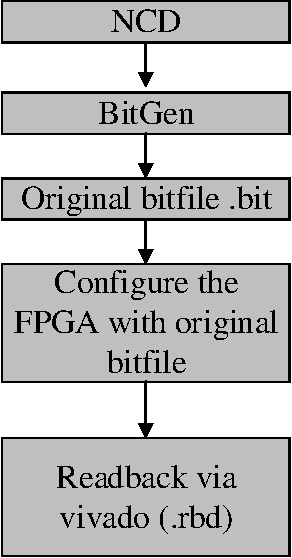
\includegraphics[scale = 0.5]{Figures/original-rbd.pdf}
   \caption{Procedure to extract the original .rbd file}
\label{fig:original-rbd}
\end{figure}

\begin{figure}[tb!]
 \centering
  \captionsetup{justification=centering}    
   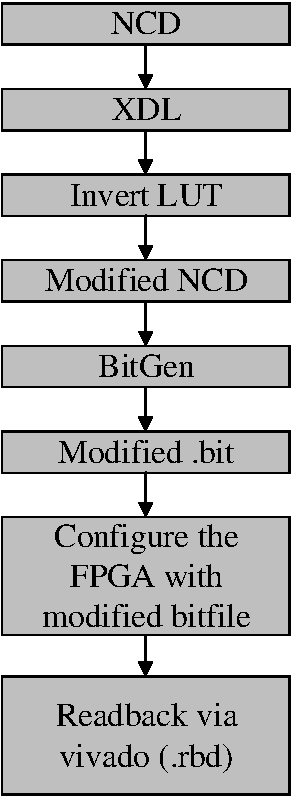
\includegraphics[scale = 0.5]{Figures/inverted-rbd.pdf}
   \caption{Procedure to extract the inverted LUT .rbd file}
\label{fig:inverted-rbd}
\end{figure}





\begin{algorithm}
\caption{Bits classification algorithm}
\begin{algorithmic}
\label{BCA}
\REQUIRE $.rbd$ $original$ $and$ $.rbd$ $inverted$ \\
%\textbf{Compute}\\ 
%\hspace{1.5cm}{$Original =  A $ $ \times $ $ B$ } \\
%\hspace{1.5cm}{$Faulty =  A $ $ \times $ $ B$ } \\
%\vspace{0.20 cm }
%\textbf{Stuck-at-1:}
\vspace{0.20 cm }

\IF{$Original$  $ = $ $ 0 $  $Inverted$ $==$ $0$}
\vspace{0.10 cm }

\STATE \textit{ NL0 = Not LUT bits at 0}
\vspace{0.10 cm }

\ELSIF{$Original$  $ = $ $ 0 $  $Inverted$ $==$ $1$}
\vspace{0.10 cm }

\STATE \textit{ L0 = LUT bits at 0}
\vspace{0.10 cm }

\ELSIF{$Original$  $ = $ $ 1 $  $Inverted$ $==$ $0$}
\vspace{0.10 cm }

\STATE \textit{ L1 =  LUT bits at 1}
\vspace{0.10 cm }

\ELSIF{$Original$  $ = $ $ 1 $  $Inverted$ $==$ $1$}
\vspace{0.10 cm }

\STATE \textit{ NL1 = Not LUT bits at 1}
\vspace{0.10 cm }




\ENDIF
\vspace{0.20 cm }

\end{algorithmic}
\end{algorithm}

















\section{Experimental Results}
\label{Experimental Results}


As mentioned in the section~\ref{intro} the main purposes of this work, is to derive the result on the realistic fault emulation environment. In this section, we will discuss the result for the fault emulation based on the emulation performed by flipping the bits state at "1", and by flipping the bits state at "0." We experimented with the fifty different runs. Each run provides $6,144$ signatures sub-divided into three separate groups.  The fault generation list is generated from the \textit{.rbd} file, extract the number of zeros and ones from the \textit{.rbd} file. Fault list randomization is being performed separately for flip-at-1 and flip-at-0 to distribute the probability of all bits to flip equally. 

Table~\ref{AE}, and Table~\ref{ME} show the percentage of the zero signature, e.g., $00000000$ for adder and multiplier. The maximum number of zero signature observed for flip-at-0. The number of bits flipped observed; $65,750$ among them $150$ bits are critical bits with the statistical ratio of $0.22\%$ critical bits. The minimum number of zero signature observed for bits flip-at-1, with the total flipped bits are $1,356$ among $3,110,418$ non-BRAM bits. In this case, the critical bits at $1$ are $11.06\%$. 

Similarly, for the multiplier,  The number of bits flipped observed are $29,752$ with total non-BRAM(bits-at-0) are $56,771,430$ giving the statistical ratio of $0.50\%$ critical bits. The minimum number of zero signature observed for bits flip-at-1, with the total flipped bits are $1,664$ among $3,750,970$ non-BRAM bits. In this case, the critical bits at $1$ are $9.01\%$.


We also performed the emulation with the random fault injection, in which we randomly combined the bits-at-1, and the bits-at-0 and calculated the zero signature. As expected, the random injection zero-signature value should lower than the flip-at-0 and higher than the flip-at-1. The purpose of performing the random injection is to compare the result with the relative sensitivity results and experimentally prove that our asymmetric SRAM cell sensitivity theory. The bit flip ratio observed in the random injection (flip-at-0 to flip-at-1) is $18.10$ for the adder as shown in Table~\ref{RI} and $15.15$ for the multiplier as shown in Table\ref{RIM}. This bit-flip information indicates that the bit flip in random mode is valid. Next, we performed the relative sensitivity experiment named SA-01, and SA-02.

In SA-01, we used the relative sensitivity concept that the  bits-at-1 are $2.11$ times more sensitive than the bit-at-0. In this emulation, we get the $1.87\%$ difference with the irradiation experiment for the adder and $1.58\%$ for the multiplier. The total bit flips we observed for adder are: $9,807$ among them $8,797$ flipped-at-0 and $1,010$ for flipped-at-1. Similarly, for the multiplier, the total bits flipped are $7,227$ among them $6,345$ flipped-at-0 and $882$ flipped-at-1. Both emulations give us the bit flipped ratio of $2.11$ proved that emulation setup is valid.

\begin{table}[tb!]
\center
\caption{Adder Emulation Tests Comparison.}

\label{AE}

\begin{tabular}{|c | c| c | c| c| c |} 
 \hline
Test & Zero Signature (\%) & Difference with Radiation (\%)   \\ 
\hline

 
 
 Flip@1& 49.048 &22.53   \\
 \hline
 Flip@0 & 62.801 & 2.095 \\ 
 \hline
 
 Random & 59.378 & 3.51  \\
 \hline
 SA-01 & 60.36 & 1.87 \\
 \hline
 SA-02 & 60.559 &1.47  \\
 \hline
 Radiation & 61.499 & 0  \\
 \hline
 
 
\end{tabular}
\end{table}


\begin{table}[tb!]
\center
\caption{Multiplier Emulation Tests Comparison.}

\label{ME}

\begin{tabular}{|c | c| c | c| c| c |} 
 \hline
Test & Zero Signature (\%) & Difference with Radiation (\%)   \\ 
\hline

 
 
 Flip@1& 62.069 &18.35   \\
 \hline
 Flip@0 & 76.066 & 1.93 \\ 
 \hline
 
 Random & 72.179 & 3.31  \\
 \hline
 SA-01 & 73.443 & 1.58 \\
 \hline
 SA-02 & 74.988 &  0.50\\
 \hline
 Radiation & 74.610 & 0  \\
 \hline
 
 
\end{tabular}
\end{table}



%We categorize the experiment in the five different categories based on the bits status, i.e., flipping the ( bits-at-1, bits-at-0, random, sensitivity based investigation that ones are more sensitive than zeros, and sensitivity based experiment consider bits feature). 
%Our emulation process is fundamentally different from the previous work published by our research group. The previous work was based on Viretx-V and fault injection was based on \textit{.ebc}, whereas this work is based on 
%the Artix-7 and fault emulation based on the \textit{.rbd} file details mentioned in section~\ref{SE-bits}. Inorder to do the fault emulation, we performed the experiment that reduce the time and the cost to perform the SEU emulation.




\begin{table}[tb!]
\center
\caption{Adder Random Injection Bits Information}

\label{RI}

\begin{tabular}{c c  c c   } 
 \hline
\multicolumn{2}{c}{Bit}     & Flip Ratio (Theoretical) &  Flip Ratio (Observed)   \\ 
%\hline
%& \multicolumn{1}{c}{ (Theoretical)} \\
%& & \multicolumn{1}{c}{observed} \\
 \hline
 
 Bits@0 & $57 411 982  $ & \multirow{2}{*}{18.45} & \multirow{2}{*}{18.10} \\
 %\hline
 Bits@1 & $3110418$  & &\\ 
 \hline
% 
% Bits@0 LUT & 2.06 &2.08 &2.096\\
% \hline
% Bits@1 LUT & 1.91 &1.92&1.91\\
 %\hline

% \hline
 
 
\end{tabular}
\end{table}


\begin{table}[tb!]
\center
\caption{Multiplier Random Injection Bits Information}

\label{RIM}

\begin{tabular}{c c  c c   } 
 \hline
\multicolumn{2}{c}{Bit}     & Flip Ratio (Theoretical) &  Flip Ratio (Observed)   \\ 
%\hline
%& \multicolumn{1}{c}{ (Theoretical)} \\
%& & \multicolumn{1}{c}{observed} \\
 \hline
 
 Bits@0 & $57 411 982  $ & \multirow{2}{*}{15.93} & \multirow{2}{*}{15.15} \\
 %\hline
 Bits@1 & $3110418$  & &\\ 
 \hline
% 
% Bits@0 LUT & 2.06 &2.08 &2.096\\
% \hline
% Bits@1 LUT & 1.91 &1.92&1.91\\
 %\hline

% \hline
 
 
\end{tabular}
\end{table}





Then, we further investigated the bits feature, i.e., bits belong to LUT and non-LUT bits. We used the bits relative sensitivity values shown in Table~\ref{RS}. The result we obtained by using this approach indicates only $1.47\%$ difference for adder and $0.50\%$ for multiplier suggest that by considering bits sensitivity with bits feature more realistic results can be achieved, and better fault emulation can be performed. 



%\begin{table}[tb!]
%\center
%\caption{Adder Emulation Tests Comparison.}
%
%\label{AE}
%
%\begin{tabular}{|c | c| c | c| c| c |} 
% \hline
%Test & Zero Signature (\%) & Difference with Radiation (\%)   \\ 
%\hline
%
% 
% 
% Flip@1& 49.048 &22.53   \\
% \hline
% Flip@0 & 62.801 & 2.095 \\ 
% \hline
% 
% Random & 59.378 & 3.51  \\
% \hline
% SA-01 & 60.36 & 1.87 \\
% \hline
% SA-02 & 60.559 &1.47  \\
% \hline
% Radiation & 61.499 & 0  \\
% \hline
% 
% 
%\end{tabular}
%\end{table}












We also measure the relative sensitivity (observed) and the bit flip information observed for this emulation setup shown in the Table~\ref{RS} to prove the bit flip emulation validity. Table~\ref{RSflipA} and~\ref{RSflipM} shows the bit flip information for the adder and multiplier respectively.


\begin{table}[tb!]
\center
\caption{Relative Sensitivity}

\label{RS}
\begin{tabular}{|c | c| c | c | } 
 \hline
Bits feature & \makecell*{Relative Sensitivity}  & \makecell*{Adder \\(Observed)} & \makecell*{Multiplier \\ (Observed)}  \\ 
%\hline
%& \multicolumn{1}{c}{ (Theoretical)} \\
%& & \multicolumn{1}{c}{observed} \\
 \hline
 
 Bits@0 non LUT & 1.00 & 1.00 & 1.00 \\
 \hline
 Bits@1 non LUT& 1.41  & 1.43&1.44\\ 
 \hline
 
 Bits@0 LUT & 2.06 &2.08 &2.09\\
 \hline
 Bits@1 LUT & 1.91 &1.92&1.91\\
 \hline

% \hline
 
 
\end{tabular}
\end{table}


















\begin{table}[tb!]
\center
\caption{Bit Flip Ratio Relative Sensitivity (Adder)}

\label{RSflipA}
\begin{tabular}{|c | c| c | c | } 
 \hline
Bits feature & \makecell*{Bit Flip)}  & \makecell*{Bit Flip Ratio\\(Total)} \\ 
%\hline
%& \multicolumn{1}{c}{ (Theoretical)} \\
%& & \multicolumn{1}{c}{observed} \\
 \hline
 
 Bits@0 non LUT & 5251  & 1.00  \\
 \hline
 Bits@1 non LUT& 236  & 1.43\\ 
 \hline
 
 Bits@0 LUT & 266 &2.08 \\
 \hline
 Bits@1 LUT & 245 &1.92\\
 \hline

% \hline
 
 
\end{tabular}
\end{table}



\begin{table}[tb!]
\center
\caption{Bit Flip Ratio Relative Sensitivity (Mull)}

\label{RSflipM}
\begin{tabular}{|c | c| c | c | } 
 \hline
Bits feature & \makecell*{Bit Flip}  & \makecell*{Bit Flip Ratio\\(Total)} \\ 
%\hline
%& \multicolumn{1}{c}{ (Theoretical)} \\
%& & \multicolumn{1}{c}{observed} \\
 \hline
 
 Bits@0 non LUT & 8833  & 1.00  \\
 \hline
 Bits@1 non LUT& 454  & 454\\ 
 \hline
 
 Bits@0 LUT & 603 &2.09\\
 \hline
 Bits@1 LUT & 553 &1.91\\
 \hline

% \hline
 
 
\end{tabular}
\end{table}







%
%\begin{equation}
%\label{eq:2}
%
%d
%\end{equation}

% \[
%    \text{Relative Sensitivity} =  \frac{x+y}{1 + \frac{y}{z+1}}
%\]

%\begin{equation} \label{eq:1}
%
%
%{Relative Sensitivity
%
%\end{equation}




%%\section{Fault Modeling}
%
%Once we get the signature from the emulation, validate all the bits flip information and zero signature validation.Next target is to drive a mathematical expression or model that can represent the high-level model that correspondence the low-level circuit faulty outputs. This model helps the designer to analyze the circuit and propose the necessary mitigation techniques at the earlier stage of the design. 
%
%
%
%\begin{algorithm}
%\caption{Generate a High-level Model of  Adder in Simulink}
%\begin{algorithmic}
%\REQUIRE $0\leq i \geq16$ \\
%\textbf{Compute}\\ 
%\hspace{1.5cm}{$Original =  A $ $ $+$ $ $ B$ } \\
%\hspace{1.5cm}{$Faulty =  A $ $ $+$ $ $ B$ } \\
%\vspace{0.20 cm }
%\textbf{Stuck-at-1:}
%\vspace{0.20 cm }
%
%\IF{$Original(i) == 1$ $and$  $Faulty (i) == 0 $}
%\vspace{0.10 cm }
%\STATE $Signature \leftarrow  \{$+$ 2^{i},$ $ $$zeros$$\{i-1\}\}$
%\vspace{0.10 cm }
%\ENDIF
%\vspace{0.20 cm }
%
%\textbf{Stuck-at-0:}
%\vspace{0.20 cm }
%\IF{$Original(i) == 0$ $and$  $Faulty (i) == 1 $}
%\vspace{0.10 cm }
%\STATE $Signature \leftarrow  \{$-$ 2^{i},$ $ $$zeros$$\{i-1\}\}$
%\vspace{0.10 cm }
%\ENDIF
%
%
%
%\vspace{0.20 cm }
%
%%\textbf{Stuck-at-0:}
%\vspace{0.20 cm }
%\IF {$Original$$-$$Faulty$  $==$ $MSB=1$ $and$ $1$}
%\vspace{0.10 cm }
%\STATE $Signature \leftarrow  \{$$Original-Faulty$$\}$
%\vspace{0.10 cm }
%\ENDIF
%
%
%
%
%%%\STATE $N \leftarrow -n$
%%%\ELSE
%%\STATE $X \leftarrow x$
%%\STATE $N \leftarrow n$
%%\ENDIF
%%\WHILE{$N \neq 0$}
%%\IF{$N$ is even}
%%\STATE $X \leftarrow X \times X$
%%\STATE $N \leftarrow N / 2$
%%\ELSE[$N$ is odd]
%%\STATE $y \leftarrow y \times X$
%%\STATE $N \leftarrow N - 1$
%%\ENDIF
%%\ENDWHILE
%\end{algorithmic}
%\end{algorithm}
%
%
%\begin{algorithm}
%\caption{Generate a High-level Model of  Multiplier in Simulink}
%\begin{algorithmic}
%\REQUIRE $ i = 16$  $bit$ $unsigned$ \\
%\textbf{Compute}\\ 
%\hspace{1.5cm}{$Original =  A $ $ \times $ $ B$ } \\
%\hspace{1.5cm}{$Faulty =  A $ $ \times $ $ B$ } \\
%\vspace{0.20 cm }
%\textbf{Stuck-at-1:}
%\vspace{0.20 cm }
%
%\IF{$Original$  $ - $  $Faulty$ $==$+$2^{i}$}
%\vspace{0.10 cm }
%\STATE $Signature \leftarrow  \{$+$ 2^{i}\}$
%\vspace{0.10 cm }
%%\ENDIF
%\vspace{0.20 cm }
%
%
%\ELSIF{$Original$  $ - $  $Faulty$ $==$ +$A$ $\times$ $2^{i}$ $or$ $ $+$B$ $\times$ $2^{i}$}
%\vspace{0.10 cm }
%\STATE $Signature \leftarrow  \{$+$  $A$ $ $ \times $ $2^{i} $ $ $or$ $ $ $+$ $B$ $ $ \times $ $2^{i}\}$
%
%
%\vspace{0.10 cm }
%\ENDIF
%\vspace{0.20 cm }
%
%\vspace{0.20 cm }
%\textbf{Stuck-at-0:}
%\vspace{0.20 cm }
%
%\IF{$Original$  $ - $  $Faulty$ $==$ -$2^{i}$}
%\vspace{0.10 cm }
%\STATE $Signature \leftarrow  \{$-$ 2^{i}\}$
%\vspace{0.10 cm }
%%\ENDIF
%\vspace{0.20 cm }
%
%
%\ELSIF{$Original$  $ - $  $Faulty$ $==$ -$A$ $\times$ $2^{i}$ $or$ $ $-$B$ $\times$ $2^{i}$}
%\vspace{0.10 cm }
%\STATE $Signature \leftarrow  \{$-$  $A$ $ $ \times $ $2^{i} $ $ $or$ $ $ $-$  $B$ $ $ \times $ $2^{i}\}$
%
%\vspace{0.10 cm }
%\ENDIF
%\vspace{0.20 cm }
%
%\end{algorithmic}
%\end{algorithm}
%
%\subsection{Adder Signature Fault Model}
%
%The adder is comprised of two 16-bits number. The adder signature is the 16-bit hexadecimal format with sign extension. The hexadecimal value comprises: first four from left are the signature hexadecimal representation, and the rest represent sign extension. The signature values with this simple expression shown in Table~\ref{adder signature format}.
%
%
%
%\begin{table}
%\center
%\caption{Adder Signature Format.}
%
%\label{adder signature format}
%
%\begin{tabular}{|c | c |} 
% \hline
%Decimal Format & Hexadecimal   \\ 
%\hline
%
% 
% 
% $16$& $00000010$    \\
% \hline
% $64$ & $00000040$  \\ 
% \hline
% 
% $128$ & $00000080$  \\
% \hline
% $-1024$ & $FFFFFC00$ \\
% \hline
% $-512$ & $FFFFFE00$ \\
% \hline
% $-8$ & $FFFFFFF8$   \\
% \hline
% 
% 
%\end{tabular}
%\end{table}
%
%
%
%
%\begin{equation}
%\label{eq:2}
%\pm±2\textsuperscript{i}    \hspace{0.5 cm} 0\leq i \geq15
%\end{equation}
%
%The Equation \ref{eq:2} can represent the adder high-level fault model. By using this equation, we can capture 99.99 \% of the signature. Table~\ref{adder signature format} shows two kinds of signature; positive signature and negative signature. The positive signature values can be modeled as \textbf{single stuck-at-one} model fault affecting an adder output bit $i$,  it adds $0$ when the target bit is at $1$ (flipped to $0$ in the faulty output). The signature computed can be expressed as $+2^{i}$. Consider the following example:
%
%
%%\rule{\linewidth}{1 pt} % A
%%\vskip-\baselineskip\vskip1.5pt % A+B
%%\rule{\linewidth}{0.1pt} %B
%\vspace{ 0.1 cm}
%\hspace{-0.3 cm}\textbf{Example:}
%\hrule height 2pt width \hsize \kern 1pt \hrule width \hsize height 1pt
%
%\vspace{0.2 cm}
%$Original$ $=$ $24$; $binary $ $ equivalent$ $11000$ \\
%
%\hspace{-0.15cm} $Faulty$ $=$ $8$; $binary $ $ equivalent$ $01000$ \\
%
%$fourth$ $bit$ $flipped$ $from$ $"1"$ $to$ $"0"$
%
%$By$ $using$ $equation$ \ref{eq:1}: \\
%
%$signature$ $=$ $8$ - $24$ $==$ $8$ $+$ $(-24)$ $=$ $16$ \\
%
%$4^{th}$ $ bit $ $flipped$; $i$  $=$ $4$, $2^{4}$ $=$ $16$
%\vspace{0.01cm}
%\hrule height 2pt width \hsize \kern 1pt \hrule width \hsize height 1pt
%
%\vspace{0.25 cm}
%
%Similarly, for the negative signature values can be modeled as single stuck-at zero model - fault affecting an adder output bit $i$, it adds $0$ when the target bit is at $0$ (flipped to $1$ in the faulty output), it adds $-2i$ to the adder output. We also observed that few signatures that didn't follow the rule number one could be modeled with: 
%
%Rule 2: if the signature cannot be modeled with the Equation~\ref{eq:1}, if the arithmetic signature values expressed in binary format and contained exactly two bits@1, including one at the MSB.
%
%\hspace{-0.3 cm}\textbf{Example valid signatures for rule \# 02:}
%\hrule height 2pt width \hsize \kern 1pt \hrule width \hsize height 1pt
%\begin{center}
%$1010 0000 0000 0000$ \\
%$1000 1000 0000 0000$ \\
%$1000 1000 0000 0000$ \\
%$1000 0000 0000 0100$ \\
%$1000 0000 0000 0001$ \\
%\end{center}
%\hrule height 2pt width \hsize \kern 1pt \hrule width \hsize height 1pt
%
%
%
%
%
%
%
%
%\subsection{Multiplier Signature Fault Model}
%
%For the 8 - bit multiplier two modeling rules have been formulated:
%
%\textbf{Rule \# 01:} This rule defines the signature can be expressed by the Equation \ref{eq:1} that represent the stuck-at-1 and stuck-at-0 fault model, when the multiplier behaves as the bit flipped occur at the output of the multiplier. 
%
%\textbf{Rule \# 02:}The rule number two defines the format of the signature obtained when a bit flipped cause the multiplier to behave as if when an input bit is either stuck-at-0 or stuck-at-1 can be represented \{$-$$A$ $\times$ $2^{i}$ $or$  $-$$B$ $\times$ $2^{i}$ \}, \{$+$$A$ $\times$ $2^{i}$ $or$  $+$$B$ $\times$ $2^{i}$ \} respectively.
\section{Conclusions}


The ultimate objective of this work is to implement a pre-certification strategy.
A sophisticated evaluation of the robustness of the designs implemented in the
SRAM-based FPGAs before sending them to the costly phase of
certification. The new technique of injecting faults by emulation is evolved.  The results obtained have illustrated that the content of the bits of
configuration has a significant impact on the type of events observed. 


In this work, sensitivity of the configuration bits has been considered along with the bits feature to
produce results as close as possible to those obtained by the accelerated tests. 



\label{Conclusion}

